% Options for packages loaded elsewhere
\PassOptionsToPackage{unicode}{hyperref}
\PassOptionsToPackage{hyphens}{url}
%
\documentclass[oneside,openany]{book}
\usepackage{amsmath,amssymb}
\usepackage{iftex}
\usepackage{listings}
\usepackage{xcolor} % For custom colors
\usepackage{hyperref}

\hypersetup{
    colorlinks=true, % Enable colored links
    linkcolor=blue,  % Color of internal links (e.g., Table of Contents)
    filecolor=magenta, % Color of file links
    urlcolor=cyan,   % Color of external hyperlinks
    citecolor=green, % Color of citation links
}


\lstset{
    language=R,                      % Set language to R
    basicstyle=\ttfamily\footnotesize, % Set font style and size
    keywordstyle=\color{blue},       % Keywords in blue
    commentstyle=\color{green!60!black}, % Comments in green
    stringstyle=\color{red},         % Strings in red
    numbers=left,                    % Line numbers on the left
    numberstyle=\tiny,               % Line number font size
    stepnumber=1,                    % Line number increment
    numbersep=5pt,                   % Distance of line numbers from the code
    backgroundcolor=\color{gray!10}, % Light gray background
    frame=single,                    % Add a frame around the code
    rulecolor=\color{black},         % Frame border color
    breaklines=true,                 % Enable line wrapping
    captionpos=b,                    % Caption at the bottom
    escapeinside={(*@}{@*)},         % For escaping into LaTeX
    morekeywords={*,...}             % Add custom R keywords if needed
}

\ifPDFTeX
  \usepackage[T1]{fontenc}
  \usepackage[utf8]{inputenc}
  \usepackage{textcomp} % provide euro and other symbols
\else % if luatex or xetex
  \usepackage{unicode-math} % this also loads fontspec
  \defaultfontfeatures{Scale=MatchLowercase}
  \defaultfontfeatures[\rmfamily]{Ligatures=TeX,Scale=1}
\fi
\usepackage{lmodern}
\ifPDFTeX\else
  % xetex/luatex font selection
\fi
% Use upquote if available, for straight quotes in verbatim environments
\IfFileExists{upquote.sty}{\usepackage{upquote}}{}
\IfFileExists{microtype.sty}{% use microtype if available
  \usepackage[]{microtype}
  \UseMicrotypeSet[protrusion]{basicmath} % disable protrusion for tt fonts
}{}
\makeatletter
\@ifundefined{KOMAClassName}{% if non-KOMA class
  \IfFileExists{parskip.sty}{%
    \usepackage{parskip}
  }{% else
    \setlength{\parindent}{0pt}
    \setlength{\parskip}{6pt plus 2pt minus 1pt}}
}{% if KOMA class
  \KOMAoptions{parskip=half}}
\makeatother
\usepackage{xcolor}
\usepackage[margin=1in]{geometry}
\usepackage{color}
\usepackage{fancyvrb}
\newcommand{\VerbBar}{|}
\newcommand{\VERB}{\Verb[commandchars=\\\{\}]}
\DefineVerbatimEnvironment{Highlighting}{Verbatim}{commandchars=\\\{\}}
% Add ',fontsize=\small' for more characters per line
\usepackage{framed}
\definecolor{shadecolor}{RGB}{248,248,248}
\newenvironment{Shaded}{\begin{snugshade}}{\end{snugshade}}
\newcommand{\AlertTok}[1]{\textcolor[rgb]{0.94,0.16,0.16}{#1}}
\newcommand{\AnnotationTok}[1]{\textcolor[rgb]{0.56,0.35,0.01}{\textbf{\textit{#1}}}}
\newcommand{\AttributeTok}[1]{\textcolor[rgb]{0.13,0.29,0.53}{#1}}
\newcommand{\BaseNTok}[1]{\textcolor[rgb]{0.00,0.00,0.81}{#1}}
\newcommand{\BuiltInTok}[1]{#1}
\newcommand{\CharTok}[1]{\textcolor[rgb]{0.31,0.60,0.02}{#1}}
\newcommand{\CommentTok}[1]{\textcolor[rgb]{0.56,0.35,0.01}{\textit{#1}}}
\newcommand{\CommentVarTok}[1]{\textcolor[rgb]{0.56,0.35,0.01}{\textbf{\textit{#1}}}}
\newcommand{\ConstantTok}[1]{\textcolor[rgb]{0.56,0.35,0.01}{#1}}
\newcommand{\ControlFlowTok}[1]{\textcolor[rgb]{0.13,0.29,0.53}{\textbf{#1}}}
\newcommand{\DataTypeTok}[1]{\textcolor[rgb]{0.13,0.29,0.53}{#1}}
\newcommand{\DecValTok}[1]{\textcolor[rgb]{0.00,0.00,0.81}{#1}}
\newcommand{\DocumentationTok}[1]{\textcolor[rgb]{0.56,0.35,0.01}{\textbf{\textit{#1}}}}
\newcommand{\ErrorTok}[1]{\textcolor[rgb]{0.64,0.00,0.00}{\textbf{#1}}}
\newcommand{\ExtensionTok}[1]{#1}
\newcommand{\FloatTok}[1]{\textcolor[rgb]{0.00,0.00,0.81}{#1}}
\newcommand{\FunctionTok}[1]{\textcolor[rgb]{0.13,0.29,0.53}{\textbf{#1}}}
\newcommand{\ImportTok}[1]{#1}
\newcommand{\InformationTok}[1]{\textcolor[rgb]{0.56,0.35,0.01}{\textbf{\textit{#1}}}}
\newcommand{\KeywordTok}[1]{\textcolor[rgb]{0.13,0.29,0.53}{\textbf{#1}}}
\newcommand{\NormalTok}[1]{#1}
\newcommand{\OperatorTok}[1]{\textcolor[rgb]{0.81,0.36,0.00}{\textbf{#1}}}
\newcommand{\OtherTok}[1]{\textcolor[rgb]{0.56,0.35,0.01}{#1}}
\newcommand{\PreprocessorTok}[1]{\textcolor[rgb]{0.56,0.35,0.01}{\textit{#1}}}
\newcommand{\RegionMarkerTok}[1]{#1}
\newcommand{\SpecialCharTok}[1]{\textcolor[rgb]{0.81,0.36,0.00}{\textbf{#1}}}
\newcommand{\SpecialStringTok}[1]{\textcolor[rgb]{0.31,0.60,0.02}{#1}}
\newcommand{\StringTok}[1]{\textcolor[rgb]{0.31,0.60,0.02}{#1}}
\newcommand{\VariableTok}[1]{\textcolor[rgb]{0.00,0.00,0.00}{#1}}
\newcommand{\VerbatimStringTok}[1]{\textcolor[rgb]{0.31,0.60,0.02}{#1}}
\newcommand{\WarningTok}[1]{\textcolor[rgb]{0.56,0.35,0.01}{\textbf{\textit{#1}}}}
\usepackage{longtable,booktabs,array}
\usepackage{calc} % for calculating minipage widths
% Correct order of tables after \paragraph or \subparagraph
\usepackage{etoolbox}
\makeatletter
\patchcmd\longtable{\par}{\if@noskipsec\mbox{}\fi\par}{}{}
\makeatother
% Allow footnotes in longtable head/foot
\IfFileExists{footnotehyper.sty}{\usepackage{footnotehyper}}{\usepackage{footnote}}
\makesavenoteenv{longtable}
\usepackage{graphicx}
\makeatletter
\def\maxwidth{\ifdim\Gin@nat@width>\linewidth\linewidth\else\Gin@nat@width\fi}
\def\maxheight{\ifdim\Gin@nat@height>\textheight\textheight\else\Gin@nat@height\fi}
\makeatother
% Scale images if necessary, so that they will not overflow the page
% margins by default, and it is still possible to overwrite the defaults
% using explicit options in \includegraphics[width, height, ...]{}
\setkeys{Gin}{width=\maxwidth,height=\maxheight,keepaspectratio}
% Set default figure placement to htbp
\makeatletter
\def\fps@figure{htbp}
\makeatother
\setlength{\emergencystretch}{3em} % prevent overfull lines
\providecommand{\tightlist}{%
  \setlength{\itemsep}{0pt}\setlength{\parskip}{0pt}}
\setcounter{secnumdepth}{5}
\ifLuaTeX
  \usepackage{selnolig}  % disable illegal ligatures
\fi
\usepackage{bookmark}
\IfFileExists{xurl.sty}{\usepackage{xurl}}{} % add URL line breaks if available
\urlstyle{same}
\hypersetup{
  pdftitle={Data Analysis Activities},
  pdfauthor={Asal Aslemand and Jaiditya Dev},
  hidelinks,
  pdfcreator={LaTeX via pandoc}}

\title{Data Analysis Activities}
\author{Asal Aslemand and Jaiditya Dev}
\date{2024-12-03}

\begin{document}
\begin{titlepage}
    \centering
    {\Huge \bfseries Data Analysis Activities\par}
    \vspace{2cm}
    {\Large Asal Aslemand and Jaiditya Dev\par}
    {\Large University of Toronto, Mississauga}
    \vfill
\end{titlepage}

\newpage
{
\setcounter{tocdepth}{2}
\tableofcontents
}
\newpage
\chapter*{Introduction}
\addcontentsline{toc}{chapter}{Introduction}


\begin{center}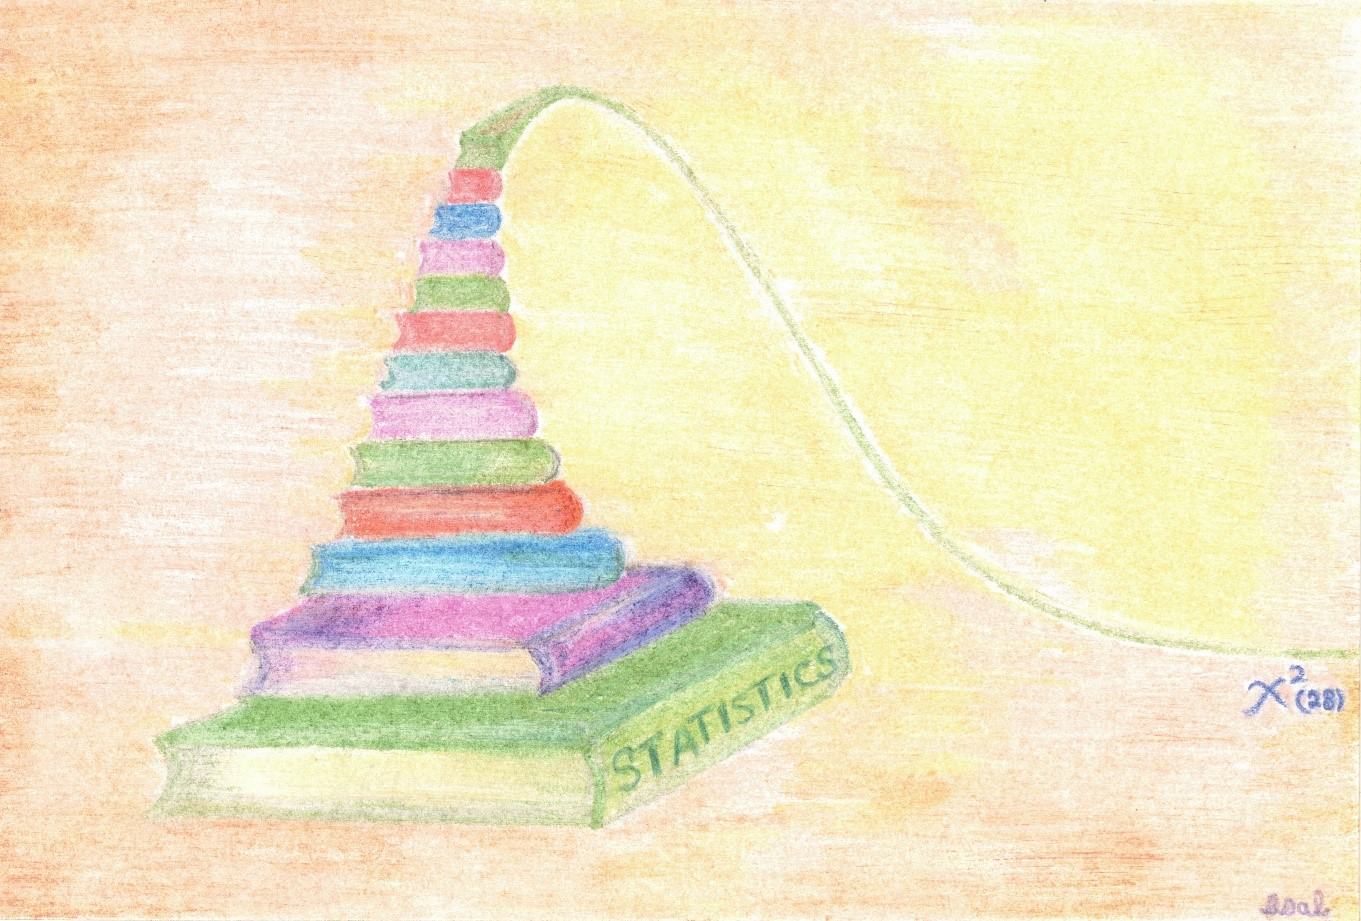
\includegraphics[width=0.65\linewidth]{Chi-square} \end{center}

This book contains a variety of statistical activities using real-life data sets. It is intended for developing statistical reasoning at an introductory to an intermediate level by explaining patterns in the data, interpreting and communicating results within the context of data, and making data-based arguments and inference. Each chapter corresponds to one statistical activity with a set of learning objectives.

Click on a link below to access a specific statistical activity.

\begin{itemize}
\tightlist
\item
  \hyperref[activity-1---exploring-categorical-data]{\textcolor{blue}{Activity 1 - Exploring Categorical Data}}
\item
  \hyperref[activity-2---exploring-quantitative-data]{\textcolor{blue}{Activity 2 - Exploring Quantitative Data}}
\item
  \hyperref[activity-3---sampling-distributions-related-to-the-normal-population]{\textcolor{blue}{Activity 3 - Sampling Distributions Related to the Normal Population}}
\item
  \hyperref[activity-4---applications-of-limit-theorem]{\textcolor{blue}{Activity 4 - Applications of Limit Theorem}}
\item
  \hyperref[activity-5---estimation-with-confidence-intervals]{\textcolor{blue}{Activity 5 - Estimation with Confidence Intervals}}
\item
  \hyperref[activity-6---introduction-to-hypothesis-testing-and-concepts]{\textcolor{blue}{Activity 6 - Introduction to Hypothesis Testing and Concepts}}
\item
  \hyperref[activity-7---errors-in-tests-statistical-power-and-sample-size]{\textcolor{blue}{Activity 7 - Errors in Tests, Statistical Power and Sample Size}}
\item
  \hyperref[activity-8---comparing-groups]{\textcolor{blue}{Activity 8 - Comparing Groups}}
\item
  \hyperref[activity-9---analysis-of-categorical-data]{\textcolor{blue}{Activity 9 - Analysis of Categorical Data}}
\item
  \hyperref[activity-10---correlation-and-introduction-to-simple-linear-regression-model]{\textcolor{blue}{Activity 10 - Correlation and Introduction to Simple Linear Regression Model}}
\end{itemize}


\begin{center}\rule{0.5\linewidth}{0.5pt}\end{center}

\textbf{Note:} Solution to each statistical activity is shared at the instructor's discretion.

\begin{center}\rule{0.5\linewidth}{0.5pt}\end{center}

If you would like to learn how to set up R on your local computer to work on these activities, please visit the \hyperref[how-to-set-up-r-for-data-analysis-activities]{\textcolor{blue}{How to Set Up R for Data Analysis Activities}} page.

\chapter{Exploring Categorical Data}\label{activity-1---exploring-categorical-data}

\section{Activity Objective}

The objective of this module is to equip you with the following:

\begin{itemize}
    \item Use R/RStudio on a desktop/laptop to simulate confidence intervals for population parameters of interest.
    \item Construct plots and frequency tables for describing categorical data.
    \item Assess association between variables.
\end{itemize}


\section{Context of Data}\label{context-of-data}

\href{https://www23.statcan.gc.ca/imdb/p2SV.pl?Function=getSurvey&SDDS=3502}{\textcolor{blue}{\textbf{Survey of Consumer Finances} (SCF, 2013)}}
 took a random sample of 6,015 adult Canadians and collected information on their level of education and whether or not they own a home. The variables ``Education Level'' and ``Home Ownership'' are measured as follows:

\begin{enumerate}
    \item \textbf{Education Level}
    \begin{itemize}
        \item No High School Diploma
        \item High School Diploma or GED
        \item Some College
        \item College Degree
    \end{itemize}
    \item \textbf{Home Ownership}
    \begin{itemize}
        \item Yes (Owns House/Condo/Ranch/Farm/Mobile Home/etc.)
        \item No (Otherwise)
    \end{itemize}
\end{enumerate}


\begin{center}\rule{0.5\linewidth}{0.5pt}\end{center}

\section{R Setup}\label{r-setup}

To set up and use R for this activity, follow the general instructions provided here:\\
\hyperref[how-to-set-up-r-for-data-analysis-activities]{\textcolor{blue}{\textbf{How to Access and Use R for Data Analysis Activities}}}.

Once you've set up your project and loaded the provided files, proceed with the activity-specific instructions below.

\begin{center}\rule{0.5\linewidth}{0.5pt}\end{center}

\section{Activity Instructions}\label{activity-instructions}

\begin{enumerate}
\def\labelenumi{\arabic{enumi}.}
\item
  Open the R script \href{https://raw.githubusercontent.com/aslemand/Data-Analysis-Activities/main/data/Activity_1/Home_SCF2013.R}{\textcolor{blue}{\texttt{Home\_SCF2013.R}}} along with the data set \href{https://raw.githubusercontent.com/aslemand/Data-Analysis-Activities/main/data/Activity_1/Home_SCF2013.csv}{\textcolor{blue}{\texttt{Home\_SCF2013.csv}}} and run it line by line in RStudio.
\item
  Examine the data using the \texttt{str()} function to understand its structure and variable names.
\item
  Generate and interpret bar plots to visualize the relationship between education level and home ownership.
\item
  Modify the bar plot code (lines 124 to 143) to include your last name in the title:

\begin{Shaded}
\begin{Highlighting}[]
\FunctionTok{library}\NormalTok{(ggplot2)}

\CommentTok{\# Exercise.}
\CommentTok{\# We will construct a side{-}by{-}side (clustered) bar chart of the data}
\CommentTok{\# bar.plot is a name where we want to save the plot and its features}
\CommentTok{\# ggplot function will make a canvas, }
\CommentTok{\# and will make the plot ready using the data set and its variables of interest}
\NormalTok{bar.plot }\OtherTok{=} \FunctionTok{ggplot}\NormalTok{(Home2, }\FunctionTok{aes}\NormalTok{(}\AttributeTok{x =}\NormalTok{ Education\_Level, }\AttributeTok{fill =}\NormalTok{ Home\_Ownership))}
\CommentTok{\# We will add the bars to the plot of the data}
\CommentTok{\# As well, we will add the legends and position it to the right{-}hand side}
\NormalTok{bar.plot }\OtherTok{=}\NormalTok{ bar.plot }\SpecialCharTok{+} \FunctionTok{geom\_bar}\NormalTok{(}\AttributeTok{position =} \StringTok{"dodge"}\NormalTok{)}
\CommentTok{\# We will add a label to the x{-}axis, }
\CommentTok{\# We will differentiate the bars by filling in the levels of the response variable}
\CommentTok{\# We will add a title and a subtitle to the plot}
\CommentTok{\# And, we will centre the position of both the title and the subtitle}
\CommentTok{\# Modify line 140 with your last{-}name in the subtitle}
\NormalTok{bar.plot }\OtherTok{=}\NormalTok{ bar.plot }\SpecialCharTok{+} \FunctionTok{labs}\NormalTok{(}\AttributeTok{xlab =} \StringTok{"Education Level"}\NormalTok{, }\AttributeTok{fill =} \StringTok{"Home Ownership"}\NormalTok{,}
                           \AttributeTok{title =} \StringTok{"Bar Plot of Home Ownership and Education Level"}\NormalTok{, }
                           \AttributeTok{subtitle =} \StringTok{"Constructed by You"}\NormalTok{)}
\NormalTok{bar.plot }\OtherTok{=}\NormalTok{ bar.plot }\SpecialCharTok{+} \FunctionTok{theme}\NormalTok{(}\AttributeTok{plot.title=}\FunctionTok{element\_text}\NormalTok{(}\AttributeTok{hjust=}\FloatTok{0.5}\NormalTok{), }
                            \AttributeTok{plot.subtitle =} \FunctionTok{element\_text}\NormalTok{(}\AttributeTok{hjust=}\FloatTok{0.5}\NormalTok{))}
\NormalTok{bar.plot}
\end{Highlighting}
\end{Shaded}
\item
  Save the modified bar plot as a \texttt{.jpeg} or \texttt{.png} file.
\end{enumerate}

\begin{center}\rule{0.5\linewidth}{0.5pt}\end{center}

\section{Related Questions}\label{related-questions}

\begin{enumerate}
\def\labelenumi{\arabic{enumi}.}
\item
  Suppose we are interested in investigating the relationship between \textbf{home ownership} and \textbf{education level}:

  \begin{itemize}
  \tightlist
  \item
    Identify the response and explanatory variable.
  \item
    Identify the role of each variable, their type, and their scale of measurement.
  \end{itemize}
\item
  Find the marginal proportions of the response variable, convert them to percentages, and interpret.
\item
  Find the conditional proportions of the response variable for each category of the explanatory variable. Convert them to percentages and interpret.
\item
  Compute the difference between the proportion of homeownership for the ``No High School Diploma'' group and the ``College Degree'' group. Interpret this difference in context.
\item
  Compute the ratio between the proportion of homeownership for the ``No High School Diploma'' group and the ``College Degree'' group. Interpret this ratio in context.
\item
  Using data-based arguments (i.e., comparing conditional proportions), describe the relationship between the variables \textbf{``home ownership''} and \textbf{``education level''}.
\end{enumerate}

\begin{center}\rule{0.5\linewidth}{0.5pt}\end{center}

\section{Submission Instructions}\label{submission-instructions}

\begin{itemize}
\tightlist
\item
  Save your bar plot as a \texttt{.doc}, \texttt{.pdf}, \texttt{.jpeg}, or \texttt{.png} file.
\item
  Provide your file to your instructor for feedback or assessment.
\end{itemize}

\chapter{Exploring Quantitative Data}\label{activity-2---exploring-quantitative-data}

\section{Context of Data}\label{context-of-data-1}

The \href{http://www.oecd.org/about/}{\textcolor{blue}{\textbf{Organisation of Economic Cooperation and Development (OECD)}}} gathers various information regarding OECD countries and its partners to promote policies that aim to improve the economic and social well-being of people around the world. From the \textbf{Better Life Index (BLI, 2021)}, a program conducted by OECD, you will analyze a quantitative variable named \textbf{Social Network Support}. This variable reflects the percentage of males and females aged 15 years and over in 41 OECD countries who perceive their social network as having relatives or friends that they can count on to help them in times of need and trouble.

\begin{center}\rule{0.5\linewidth}{0.5pt}\end{center}

\section{R Setup}\label{r-setup-1}

To set up and use R for this activity, follow the general instructions provided here:\\
\hyperref[how-to-set-up-r-for-data-analysis-activities]{\textcolor{blue}{\textbf{How to Access and Use R for Data Analysis Activities}}}.

Once you've set up your project and loaded the provided files, proceed with the activity-specific instructions below.

\begin{center}\rule{0.5\linewidth}{0.5pt}\end{center}

\section{Activity Instructions}\label{activity-instructions-1}

\begin{enumerate}
\def\labelenumi{\arabic{enumi}.}
\item
  Open the R script \href{https://raw.githubusercontent.com/aslemand/Data-Analysis-Activities/main/data/Activity_2/Social.R}{\textcolor{blue}{\texttt{Social.R}}} and run it line by line in RStudio.
\item
  Begin by reading/importing the data file \href{https://raw.githubusercontent.com/aslemand/Data-Analysis-Activities/main/data/Activity_2/Social.csv}{\textcolor{blue}{\texttt{Social.csv}}} into R.
\item
  Examine the data structure and variables using \texttt{str()} and summary statistics functions.
\item
  Create side-by-side boxplots to compare distributions of \textbf{Social Network Support} percentages for males and females.
\item
  Modify the plot title (line 86 in the R script) to include your last name. For example:

\begin{Shaded}
\begin{Highlighting}[]
\NormalTok{box.plot }\OtherTok{\textless{}{-}}\NormalTok{ box.plot }\SpecialCharTok{+} \FunctionTok{labs}\NormalTok{(}\AttributeTok{title =} \StringTok{"Boxplot of Data Constructed by You"}\NormalTok{)}
\end{Highlighting}
\end{Shaded}
\item
  Save the boxplot as a \texttt{.jpeg} or \texttt{.png} file.
\end{enumerate}

\begin{center}\rule{0.5\linewidth}{0.5pt}\end{center}

\section{Related Questions}\label{related-questions-1}

After completing the activity, answer the following questions using your results:

\begin{enumerate}
\def\labelenumi{\arabic{enumi}.}
\tightlist
\item
  Refer to your statistical analysis of percentages of perceived social network support for males and females. Use side-by-side boxplots and summary statistics to compare the distributions. \bigbreak

  \begin{itemize}
  \tightlist
  \item
    Compare the shapes, centers, and spreads of both distributions.
  \item
    Identify potential outliers using the 1.5 IQR rule. For any outlier(s), determine how many standard deviations they are away from the overall mean of the distribution.
  \end{itemize}
\item
  Use the boxplot and summary statistics for the differences between females' and males' percentages of perceived social network support (in each country) to describe what this plot reveals that the side-by-side boxplots do not.\bigbreak

  \begin{itemize}
  \tightlist
  \item
    Discuss the shape, center, and spread of the differences.
  \item
    Identify suspect outliers using the 1.5 IQR rule and calculate their deviation from the overall mean.
  \item
    Explain why the boxplot of differences is more insightful for understanding differences between males and females across OECD countries.
  \end{itemize}
\end{enumerate}

\begin{center}\rule{0.5\linewidth}{0.5pt}\end{center}

\section{Submission Instructions}\label{submission-instructions-1}

\begin{itemize}
\tightlist
\item
  Save your boxplot of differences in percentages of perceived social support network as a \texttt{.doc}, \texttt{.pdf}, \texttt{.jpeg}, or \texttt{.png} file.
\item
  Share your file with your instructor or teaching assistant for feedback or assessment.
\end{itemize}

\chapter{Sampling Distributions Related to the Normal Population}\label{activity-3---sampling-distributions-related-to-the-normal-population}

\section{Activity Objective}\label{activity-objective}

The objective of this module is to equip you with the following:
\begin{itemize}
    \item Use R/RStudio on a desktop/laptop to simulate data from a Normal model.
    \item Describe the sampling distribution of sample means.
    \item Recognize sampling distributions related to the normal population.
\end{itemize}


\section{Context of Data}\label{context-of-data-2}

At-term newborns in Canada vary in weight according to an approximate \textbf{Normal model}, with the following parameters:
- Mean: 3500 grams
- Standard Deviation: 500 grams

The objective of this activity is to explore the sampling distributions of sample means and understand how they relate to the normal distribution.

\begin{center}\rule{0.5\linewidth}{0.5pt}\end{center}

\section{R Setup}\label{r-setup-2}

To set up and use R for this activity, follow the general instructions provided here:\\
\hyperref[how-to-set-up-r-for-data-analysis-activities]{\textcolor{blue}{\textbf{How to Access and Use R for Data Analysis Activities}}}.

Once you've set up your project and loaded the provided files, proceed with the activity-specific instructions below.

\begin{center}\rule{0.5\linewidth}{0.5pt}\end{center}

\section{Activity Instructions}\label{activity-instructions-2}

\begin{enumerate}
\def\labelenumi{\arabic{enumi}.}
\tightlist
\item
  Open the R script \href{https://raw.githubusercontent.com/aslemand/Data-Analysis-Activities/main/data/Activity_3/Newborn_Weights.R}{\textcolor{blue}{\texttt{Newborn\_Weights.R}}} and start running the provided code.
\item
  Modify the R code as follows:

  \begin{itemize}
  \tightlist
  \item
    \textbf{Line 7}: Insert a unique seed number.
  \end{itemize}

\begin{Shaded}
\begin{Highlighting}[]
\CommentTok{\# Enter your seed number in line 8.}
\FunctionTok{set.seed}\NormalTok{( )}
\end{Highlighting}
\end{Shaded}

  \begin{itemize}
  \tightlist
  \item
    \textbf{Line 39}: Add your last name to the title of the plot.
  \end{itemize}

\begin{Shaded}
\begin{Highlighting}[]
\CommentTok{\# Make a change to line 40. Include your last name in the main (title) argument.}
\FunctionTok{hist}\NormalTok{(Xbar, }
   \AttributeTok{main =} \StringTok{"Histogram of Sample Means }\SpecialCharTok{\textbackslash{}n}\StringTok{ Conducted by You"}\NormalTok{, }
   \AttributeTok{xlab =} \StringTok{"Xbar: Sample Means for Total Weights (in grams) of New Borns"}\NormalTok{, }
   \AttributeTok{col =} \StringTok{"lavender"}\NormalTok{)}
\end{Highlighting}
\end{Shaded}
\item
  Simulate 100 samples of size \(n = 30\) from the population distribution of newborn weights. Store the means in a variable named \texttt{Xbar}.
\item
  Construct a frequency histogram of the sampling distribution of sample means. Obtain summary statistics and interpret:

  \begin{itemize}
  \tightlist
  \item
    Shape
  \item
    Center
  \item
    Spread
  \end{itemize}
\item
  Experiment with other sample sizes (\(n = 2, 5, 15, 30, 100, 300\)) using different replication numbers (\(n = 1000\)):

  \begin{itemize}
  \tightlist
  \item
    Plot the sampling distributions of sample means for these sample sizes.
  \item
    Identify which sample size gives the smallest \textbf{Standard Error}.
  \end{itemize}
\end{enumerate}

\begin{center}\rule{0.5\linewidth}{0.5pt}\end{center}

\section{Related Questions}\label{related-questions-2}

After completing the activity, answer the following questions:

\begin{enumerate}
\def\labelenumi{\arabic{enumi}.}
\tightlist
\item
  \textbf{Sampling Distribution Analysis}:

  \begin{itemize}
  \tightlist
  \item
    Using the boxplot and Normal QQ plot, describe the sampling distribution of your sampled data. Justify your answer with both visualizations.
  \end{itemize}
\item
  \textbf{IQR Extrapolation}:

  \begin{itemize}
  \tightlist
  \item
    Refer to the summary statistics. Write a sentence that extrapolates the \textbf{IQR} for this sample into a statement about the population. Ensure your wording is precise.
  \end{itemize}
\item
  \textbf{Sampling Distribution of Means}:

  \begin{itemize}
  \tightlist
  \item
    For \(n = 30\), describe the sampling distribution of sample means (shape, center, and spread). Use summary statistics and histogram to support your analysis.
  \end{itemize}
\item
  \textbf{Effect of Sample Size}:

  \begin{itemize}
  \tightlist
  \item
    Compare sampling distributions for different sample sizes (\(n = 2, 5, 15, 30, 100, 300\)).
  \item
    Identify which sample size gives the smallest \textbf{Standard Error} and explain why.
  \end{itemize}
\end{enumerate}

\begin{center}\rule{0.5\linewidth}{0.5pt}\end{center}

\section{Submission Instructions}\label{submission-instructions-2}

\begin{itemize}
\tightlist
\item
  Save the histogram of the sampling distribution of sample means for newborn weights (\(n = 30\)) as a \texttt{.doc}, \texttt{.pdf}, \texttt{.jpeg}, or \texttt{.png} file.
\item
  Provide your file to your instructor or teaching assistant for feedback or assessment.
\end{itemize}

\chapter{Applications of Limit Theorem}\label{activity-4---applications-of-limit-theorem}

\section{Activity Objective}\label{activity-objective-1}

The objective of this module is to equip you with the following:
- Use R/RStudio on a desktop/laptop to construct sampling distribution of the sample mean.
- Explore the concept of central limit theorem
- Apply the Normal Approx. to the Binomial

\section{Context of Data}\label{context-of-data}

The General Social Survey (GSS, 2013) reports the total number of groups, organizations, and associations that individuals, persons 12 years of age and older in Canada, participated in during the past 12 months. A researcher took a random sample of 100 persons 12 years of age and older from this population. She asked the randomly selected persons to indicate the total number of groups, organizations, and associations that they participated in during the past 12 months. She stored her data in a CSV file and named the variable of interest ``group''.

\section{Activity Instructions}\label{activity-instructions}

Complete the following steps and work on answering the related questions:

\begin{enumerate}
\def\labelenumi{\arabic{enumi}.}
\item
  Download the following two files to your computer:

  \begin{itemize}
  \tightlist
  \item
    {\textcolor{blue}{Data File: }}\href{https://raw.githubusercontent.com/aslemand/Data-Analysis-Activities/main/data/Activity_4/Volunteering.csv}{\textcolor{blue}{Volunteering.csv}}
  \item
    {\textcolor{blue}{R Script:} }\href{https://raw.githubusercontent.com/aslemand/Data-Analysis-Activities/main/data/Activity_4/Volunteering.R}{\textcolor{blue}{Volunteering.R}}
  \end{itemize}
\item
  Follow the instructions provided on the \textbf{How to Access and Use R for Data Analysis Activities} page to set up your R environment:\\
  \hyperref[how-to-set-up-r-for-data-analysis-activities]{\textcolor{blue}{\textbf{How to Access and Use R for Data Analysis Activities}}}.
\item
  Once you've set up your project folder and uploaded the files, proceed with the steps below:

  \begin{itemize}
  \tightlist
  \item
    Open the R script \texttt{Volunteering.R} and start running the provided codes.
  \end{itemize}
\item
  There are two required R code modifications:

  \begin{itemize}
  \tightlist
  \item
    \textbf{Lines 26 to 30} require you to input a seed number into line 30. Put it into line 30 and run the line of code in R.
  \end{itemize}

\begin{Shaded}
\begin{Highlighting}[]
\CommentTok{\# R code modification \#1: Obtain sampling Distribution of Sample Means}
\CommentTok{\# Pick a seed number so that each time you run your sampling,}
\CommentTok{\# you will obtain the same result.}
\CommentTok{\# Enter your seed number in line 30.}
\FunctionTok{set.seed}\NormalTok{( ) }\CommentTok{\# Enter your seed number here}
\end{Highlighting}
\end{Shaded}

  \begin{itemize}
  \tightlist
  \item
    \textbf{Lines 40 to 45} in the R script describe a small exercise to make a change to line 43. You will insert your last name in the title of the plot. Make the change to the line mentioned and upload your plot using this assignment page.
  \end{itemize}

\begin{Shaded}
\begin{Highlighting}[]
 \CommentTok{\# R code modification \#2: Plot the Sampling Distribution of Sample Means}
 \CommentTok{\# for Total Number of Group Participation}
 \CommentTok{\# Make a change to line 43. Include your last name in the main (title) argument.}
   \FunctionTok{hist}\NormalTok{(Xbar, }
      \AttributeTok{main =} \StringTok{"Histogram of Sample Means }\SpecialCharTok{\textbackslash{}n}\StringTok{ Conducted by You"}\NormalTok{, }
      \AttributeTok{xlab =} \StringTok{"Xbar: Sample Means for Total Number of Group Participation"}\NormalTok{, }
      \AttributeTok{col =} \StringTok{"lavender"}\NormalTok{)}
\end{Highlighting}
\end{Shaded}
\end{enumerate}

\begin{center}\rule{0.5\linewidth}{0.5pt}\end{center}

\section{Related Questions}\label{related-questions-3}

Based on your R analysis (using your R outputs), answer the following related questions:

\begin{enumerate}
\def\labelenumi{\arabic{enumi}.}
\item
  Refer to the plots of data (boxplot and Normal QQ plot). Does it appear that this data could have come from a normal distribution? Use \textbf{both} plots to justify your answer.
\item
  Refer to the summary statistics of the data. Write a sentence that extrapolates the \textbf{IQR} for this sample into a statement about the population -- be careful with your wording.
\item
  Use the sample mean and sample standard deviation of the total number of group participation as the parameter values for the population mean and population standard deviation. If the population distribution of the total number of group participation was normal, 20\% of all cases in the specified age range participated in at least how many group organizations? Find \(x\).
\item
  For this question, treat the ``group'' data as a population data (\(N = 100\)). Note the mean as the population mean and SD as the population SD. Draw 60 samples of size \(n = 50\) each from this supposed population distribution to approximate the sampling distribution of sample means total number of group participation. Store the result of your experiment in a variable named \texttt{Xbar}. Construct a frequency histogram and obtain summary statistics for the sampling distribution of sample means total number of group participation. Describe the shape, center, and spread of the sampling distribution of sample means total number of group participation for 50 persons in the specified age group. Name the theorem that you use to answer this question.
\end{enumerate}

\begin{center}\rule{0.5\linewidth}{0.5pt}\end{center}

\section{Submission Instructions}\label{submission-instructions}

Using this assignment page, upload your histogram for the sampling distribution of sample means total number of group participation. The accepted file formats for  submission are \texttt{.doc}, \texttt{.pdf}, \texttt{.jpeg}, or \texttt{.png} files.

\chapter{Estimation with Confidence Intervals}\label{activity-5---estimation-with-confidence-intervals}

\section{Activity Objective}\label{activity-objective-2}

The objective of this module is to equip you with the following:
\begin{itemize}
    \item Use R/RStudio on a desktop/laptop to simulate confidence intervals for population parameters of interest.
    \item Construct a confidence interval for one mean (known sigma) from a Normal Population.
    \item Construct a confidence interval for one mean (unknown sigma, small sample) from a Normal Population.
    \item Construct a confidence interval for one proportion.
    \item Construct a confidence interval for one variance.
\end{itemize}


\begin{center}\rule{0.5\linewidth}{0.5pt}\end{center}

\section{Context of Data}\label{context-of-data}

Suppose \textbf{STA123 course grades} are Normally distributed. Instead of collecting data from students, we will simulate (generate) some data for our example. To simulate data, we need to know the population mean and standard deviation of STA123 course grades. Here we assume the mean STA123 course grades is \textbf{70} and the standard deviation is \textbf{5}.

Using the sampled data, we obtain a \textbf{95\% CI for population mean STA123 course grades}. Next, we carry out an experiment for CI interpretation. We know that a CI changes each time with a study. If we repeat the same study again and again, (1-\(\alpha\))\% of the time the obtained confidence intervals would cover the true population parameter value. This can be shown through a simulation study or experiment. Using the STA123 course grades example, we can conduct an experiment using the following steps:

\begin{enumerate}
\def\labelenumi{\arabic{enumi}.}
\tightlist
\item
  Generate a set of STA123 course grades data with 150 students from the population.
\item
  Calculate the observed sample mean of STA123 course grades and the standard error of \(\bar{X}\).
\item
  Calculate the confidence interval.
\item
  Check whether the confidence interval contains the population parameter value.
\item
  Repeat steps (1)-(4) \textbf{10,000 times} and count the total number of times that the confidence intervals contain the population value.
\item
  For a \textbf{95\% CI}, one would expect about \textbf{9500 times} the CIs contain the population value.
\end{enumerate}

Next, we draw a plot of the first 100 simulated confidence intervals and indicate those which do not contain the true population mean value of 70.

\begin{center}\rule{0.5\linewidth}{0.5pt}\end{center}

\section{Activity Instructions}\label{activity-instructions}

\begin{enumerate}
\def\labelenumi{\arabic{enumi}.}
\item
  Download the following file to your computer:

  \begin{itemize}
  \tightlist
  \item
    \href{https://raw.githubusercontent.com/aslemand/Data-Analysis-Activities/main/data/Activity_5/Interval-Estimates-Simulations.R}{\textcolor{blue}{R Script: Interval-Estimates-Simulations.R}}
  \end{itemize}
\item
  Follow the instructions provided on the \textbf{How to Access and Use R for Data Analysis Activities} page to set up your R environment:\\
  \hyperref[how-to-set-up-r-for-data-analysis-activities]{\textcolor{blue}{\textbf{How to Access and Use R for Data Analysis Activities}}}.
\item
  Once you've set up your project folder and uploaded the file, proceed with the steps below:

  \begin{itemize}
  \tightlist
  \item
    Open the R script \texttt{Interval-Estimates-Simulations.R} and start running the provided code.
  \end{itemize}
\item
  There are two required R code modifications:

  \begin{itemize}
  \tightlist
  \item
    \textbf{Line 15}: You need to input a seed number. Choose your seed number and put it into line 15 and run the line of code in R.
  \item
    \textbf{Line 96}: You need to insert your last name in the title of the plot. Make the change to this line and upload your plot using this assignment page.
  \end{itemize}
\end{enumerate}

\begin{center}\rule{0.5\linewidth}{0.5pt}\end{center}

\section{Related Questions}\label{related-questions-4}

Based on your R analysis (using your R outputs), answer the following related questions:

\begin{enumerate}
\def\labelenumi{\arabic{enumi}.}
\item
  Refer to the plots of your sampled data (histogram, boxplot, and Normal QQ plot). Describe the distribution of sampled data.
\item
  Use the results of your sampled data to construct a \textbf{95\% CI} for \(\mu\).
\item
  Briefly describe the result of your simulation. What do you observe?
\end{enumerate}

\begin{center}\rule{0.5\linewidth}{0.5pt}\end{center}

\section{Submission Instructions}\label{submission-instructions}

Using this assignment page, upload your plot of the \textbf{95\% confidence intervals} using your simulated data. The accepted file formats for  submission are \texttt{.doc}, \texttt{.pdf}, \texttt{.jpeg}, or \texttt{.png} files.

\chapter{Introduction to Hypothesis Testing and Concepts}\label{activity-6---introduction-to-hypothesis-testing-and-concepts}

\section{Activity Objective}\label{activity-objective-3}

The objective of this module is to equip you with the following:

\begin{itemize}
\tightlist
\item
  Use R/RStudio on a desktop/laptop to carry out hypothesis testing and to estimate error probability via simulation.
\item
  Employ hypothesis testing for:

  \begin{itemize}
  \tightlist
  \item
    \textbf{One Proportion}
  \item
    \textbf{One Mean}

    \begin{itemize}
    \tightlist
    \item
      Sigma known, Normal population:

      \begin{itemize}
      \tightlist
      \item
        Large sample
      \item
        Small sample
      \end{itemize}
    \item
      Sigma unknown, estimate sigma (replace with sample standard deviation):

      \begin{itemize}
      \tightlist
      \item
        Large sample, CLT applies
      \item
        Small sample, assess (or know) whether the random sample comes from a Normal population.
      \end{itemize}
    \end{itemize}
  \item
    \textbf{One Variance}

    \begin{itemize}
    \tightlist
    \item
      Independent, (small or large) random sample.
    \end{itemize}
  \end{itemize}
\end{itemize}

\begin{center}\rule{0.5\linewidth}{0.5pt}\end{center}

\section{Context of Data}\label{context-of-data}

Suppose \textbf{STA123 course grades} are Normally distributed with a mean of \textbf{70} and a standard deviation of \textbf{5}.

Estimate the error probability in a t-test of \(H_0: \mu = 70\) versus \(H_a: \mu > 70\), when the underlying population is Normal with \(\mu = 70\) and \(\sigma = 5\). Take a random sample of \(n = 25\) and test at \(\alpha = 0.05\).

Using the STA123 course grades example, we can conduct an experiment using the following steps:
1. Generate a set of \textbf{10,000} STA123 course grades data with 25 students from the population.
2. For each of the generated random samples, conduct a t-test.
3. Store the observed t-test statistics and the p-values in a matrix.
4. Count the number of p-values that are \(\leq 0.05\) (\(\alpha\)-level) to estimate the probability of error.

\begin{center}\rule{0.5\linewidth}{0.5pt}\end{center}

\section{Activity Instructions}\label{activity-instructions}

\begin{enumerate}
\def\labelenumi{\arabic{enumi}.}
\item
  Download the following file to your computer:

  \begin{itemize}
  \tightlist
  \item
    \href{https://raw.githubusercontent.com/aslemand/Data-Analysis-Activities/main/data/Activity_6/Hypothesis-Testing-Error-Probability-Simulation.R}{\textcolor{blue}{R Script: Hypothesis Testing-Error Probability-Simulation.R}}
  \end{itemize}
\item
  Follow the instructions provided on the \textbf{How to Access and Use R for Data Analysis Activities} page to set up your R environment:\\
  \hyperref[how-to-set-up-r-for-data-analysis-activities]{\textcolor{blue}{\textbf{How to Access and Use R for Data Analysis Activities}}}.
\item
  Once you've set up your project folder and uploaded the file, proceed with the steps below:

  \begin{itemize}
  \tightlist
  \item
    Open the R script \texttt{Hypothesis\ Testing-Error\ Probability-Simulation.R} and start running the provided code.
  \end{itemize}
\item
  There are two required R code modifications:

  \begin{itemize}
  \tightlist
  \item
    \textbf{Line 10}: You need to input a seed number. You are provided with a unique seed number that you can retrieve from  in your Grade page (see \hyperref[]{Seed Number}). Find your seed number and put it into line 10 and run the line of code in R.
  \end{itemize}

\begin{Shaded}
\begin{Highlighting}[]
\CommentTok{\# R code modification \#1: }
\CommentTok{\# Enter your seed number inside the function set.seed( ) }
\CommentTok{\# set.seed() function in R will create reproducible results.}
\FunctionTok{set.seed}\NormalTok{()}
\end{Highlighting}
\end{Shaded}

  \begin{itemize}
  \tightlist
  \item
    \textbf{Line 75}: You need to insert your last name in the title of the plot. Make the change to this line and upload your plot using this assignment page.
  \end{itemize}

\begin{Shaded}
\begin{Highlighting}[]
\CommentTok{\# R code modification \#2: }
\CommentTok{\# Make a change to the main (title) of the plot by adding your last name to it.}
\FunctionTok{library}\NormalTok{(ggplot2)}
\NormalTok{hist.plot }\OtherTok{=} \FunctionTok{ggplot}\NormalTok{(}\AttributeTok{data =}\NormalTok{ HT.Array) }
\NormalTok{hist.plot }\OtherTok{=}\NormalTok{ hist.plot }\SpecialCharTok{+} \FunctionTok{geom\_histogram}\NormalTok{(}\FunctionTok{aes}\NormalTok{(}\AttributeTok{x =}\NormalTok{ t.Stat,}
                                           \AttributeTok{y =} \FunctionTok{after\_stat}\NormalTok{(count }\SpecialCharTok{/} \FunctionTok{sum}\NormalTok{(count)),}
                                           \AttributeTok{fill =}\NormalTok{ P.value }\SpecialCharTok{\textless{}=} \FloatTok{0.05}\NormalTok{), }
                                       \AttributeTok{binwidth =} \FloatTok{0.5}\NormalTok{, }
                                       \AttributeTok{color =} \StringTok{\textquotesingle{}black\textquotesingle{}}\NormalTok{)}
\NormalTok{hist.plot }\OtherTok{=}\NormalTok{ hist.plot }\SpecialCharTok{+} \FunctionTok{scale\_fill\_manual}\NormalTok{(}\AttributeTok{values=}\FunctionTok{c}\NormalTok{(}\StringTok{"lightgrey"}\NormalTok{, }\StringTok{"darkorange"}\NormalTok{), }
                                          \AttributeTok{name=}\StringTok{"P.values \textless{}= 0.05"}\NormalTok{,}
                                          \AttributeTok{labels=}\FunctionTok{c}\NormalTok{(}\StringTok{"No"}\NormalTok{, }\StringTok{"Yes"}\NormalTok{))}
\NormalTok{hist.plot }\OtherTok{=}\NormalTok{ hist.plot }\SpecialCharTok{+} \FunctionTok{labs}\NormalTok{(}\AttributeTok{x =} \StringTok{"t Statistics"}\NormalTok{, }
                             \AttributeTok{y =} \StringTok{"Proportion"}\NormalTok{)}
\NormalTok{hist.plot }\OtherTok{=}\NormalTok{ hist.plot }\SpecialCharTok{+} \FunctionTok{ggtitle}\NormalTok{(}\StringTok{\textquotesingle{}Simulated t Statistics Conducted by You\textquotesingle{}}\NormalTok{)}
\NormalTok{hist.plot }\SpecialCharTok{+} \FunctionTok{theme\_bw}\NormalTok{() }\SpecialCharTok{+} \FunctionTok{theme}\NormalTok{(}\AttributeTok{plot.title=}\FunctionTok{element\_text}\NormalTok{(}\AttributeTok{hjust=}\FloatTok{0.5}\NormalTok{))}
\end{Highlighting}
\end{Shaded}
\end{enumerate}

\begin{center}\rule{0.5\linewidth}{0.5pt}\end{center}

\section{Related Questions}\label{related-questions-5}

Based on your R analysis (using your R outputs), answer the following related questions:

\begin{enumerate}
\def\labelenumi{\arabic{enumi}.}
\tightlist
\item
  Briefly describe the result of your simulation. What do you observe?
\end{enumerate}

\begin{center}\rule{0.5\linewidth}{0.5pt}\end{center}

\section{Submission Instructions}\label{submission-instructions}

Using this assignment page, upload your histogram of t-statistics based on your simulated data. The accepted file formats for  submission are \texttt{.doc}, \texttt{.pdf}, \texttt{.jpeg}, or \texttt{.png} files.

\chapter{Errors in Tests, Statistical Power and Sample Size}\label{activity-7---errors-in-tests-statistical-power-and-sample-size}

\section{Activity Objective}\label{activity-objective-4}

The objective of this module is to equip you with the following:

\begin{itemize}
    \item Obtain statistical power.
    \item Use statistical power to find sample sizes.
    \item Use R/RStudio on a desktop/laptop to explore the relationship between statistical power and sample sizes for different mean values.
\end{itemize}


\begin{center}\rule{0.5\linewidth}{0.5pt}\end{center}

\section{Context of Data}\label{context-of-data}

Suppose it is claimed that the mean STA123 course grade is 70. The population SD is 4 (suppose sigma is known). Suppose that the population distribution of STA123 course grades is Normal. Suppose we test \(H_0: \mu = 70\) versus \(H_a: \mu < 70\). Suppose the true \(\mu\) value is something else (i.e., 68). So \(H_0\) (the null hypothesis) is wrong. How likely is that to happen? This is the power of the test:

\begin{itemize}
\tightlist
\item
  In R, the function is: \texttt{power.t.test}.
\item
  The argument delta in this function is the difference between null and true mean.
\item
  We also need a sample size. Let's consider various sample sizes and their effect on power.
\item
  We will examine the relationship between power and sample sizes for different mean values (possible true \(\mu\) values).
\item
  We plot the power curves.
\end{itemize}

\section{Activity Instructions}\label{activity-instructions}

\begin{enumerate}
\def\labelenumi{\arabic{enumi}.}
\tightlist
\item
  Use Chrome or Firefox to download the following file to your computer:

  \begin{itemize}
  \tightlist
  \item
    \href{https://raw.githubusercontent.com/aslemand/Data-Analysis-Activities/main/data/Activity_7/Statistical_Power.R}{\textcolor{blue}{R Script: Statistical Power.R}}
  \end{itemize}
\item
  Follow the \hyperref[how-to-set-up-r-for-data-analysis-activities]{\textbf{How to Access and Use R for Data Analysis Activities}}. to prepare your environment.
\item
  Upload the downloaded R script into the appropriate folder in your project directory.
\item
  Open the R script and start running the provided code.
\item
  \textbf{Required R code modification}:

  \begin{itemize}
  \tightlist
  \item
    In \textbf{line 44}, you need to insert your last name in the title of the plot. Make the change to this line and upload your plot using this assignment page.
  \end{itemize}

\begin{Shaded}
\begin{Highlighting}[]
\CommentTok{\# Plot the power curve for different true mean values as n sample size increases}
\NormalTok{power.curve }\OtherTok{=} \FunctionTok{ggplot}\NormalTok{(my\_data, }\FunctionTok{aes}\NormalTok{(}\AttributeTok{x =}\NormalTok{ n, }\AttributeTok{y =}\NormalTok{ power, }\AttributeTok{colour =}\NormalTok{ mean)) }\SpecialCharTok{+}
  \FunctionTok{geom\_point}\NormalTok{() }\SpecialCharTok{+} \FunctionTok{geom\_line}\NormalTok{() }\SpecialCharTok{+}
  \FunctionTok{geom\_hline}\NormalTok{(}\AttributeTok{yintercept =} \DecValTok{1}\NormalTok{, }\AttributeTok{linetype=}\StringTok{"dashed"}\NormalTok{) }\SpecialCharTok{+} 
  \FunctionTok{xlab}\NormalTok{(}\StringTok{"sample size"}\NormalTok{) }\SpecialCharTok{+}
  \CommentTok{\# Make a change to the main (title) of the plot by adding your last name to it}
  \FunctionTok{ggtitle}\NormalTok{(}\StringTok{\textquotesingle{}Relationship Between Power and Sample Sizes for Different Mean Value}
  \StringTok{Constructed by You\textquotesingle{}}\NormalTok{) }\SpecialCharTok{+}
  \FunctionTok{theme}\NormalTok{(}\AttributeTok{plot.title=}\FunctionTok{element\_text}\NormalTok{(}\AttributeTok{hjust=}\FloatTok{0.5}\NormalTok{))}
\NormalTok{power.curve}
\end{Highlighting}
\end{Shaded}
\end{enumerate}

\begin{center}\rule{0.5\linewidth}{0.5pt}\end{center}

\section{Related Questions}\label{related-questions-6}

Based on your R analysis (using your R outputs), answer the following related question:

\begin{itemize}
\tightlist
\item
  Refer to the plot of power curves. What do you observe?
\end{itemize}

\begin{center}\rule{0.5\linewidth}{0.5pt}\end{center}

\section{Submission Instructions}\label{submission-instructions}

Using this assignment page, upload your plot of power curves. The accepted file formats for  submission are \texttt{.doc}, \texttt{.pdf}, \texttt{.jpeg}, or \texttt{.png} files.

\chapter{Comparing Groups}\label{activity-8---comparing-groups}

\section{Activity Objective}\label{activity-objective-5}

The objective of this module is to equip you with the following:
\begin{itemize}
    \item Comparing groups.
    \item Use R/RStudio in a desktop/laptop environment to test relationships between a quantitative variable and a categorical variable.
\end{itemize}


\begin{center}\rule{0.5\linewidth}{0.5pt}\end{center}

\section{Context of Data}\label{context-of-data}

Every year, the US releases to the public a large data set containing information on births recorded in the country. This data set has been of interest to medical researchers who are studying the relation between habits and practices of expectant mothers and the birth of their children. We will work with a random sample of 1,000 cases from the data set released in 2014.

We would like to know: is there convincing evidence that newborns from mothers who smoke have a different average birth weight than newborns from mothers who do not smoke? We will use data from this sample to try to answer this question.

\begin{center}\rule{0.5\linewidth}{0.5pt}\end{center}

\section{Activity Instructions}\label{activity-instructions-3}

Complete the following steps and work on answering the related question:

\begin{enumerate}
\def\labelenumi{\arabic{enumi}.}
\tightlist
\item
  \textbf{Download the R script}:

  \begin{itemize}
  \tightlist
  \item
    Download the following R script to your computer:

    \begin{itemize}
    \tightlist
    \item
      \href{https://raw.githubusercontent.com/aslemand/Data-Analysis-Activities/main/data/Activity_8/babies.R}{\textcolor{blue}{babies.R}}
    \end{itemize}
  \end{itemize}
\item
  \textbf{Set up your R environment}:

  \begin{itemize}
  \tightlist
  \item
    Follow the instructions provided on the page mentioned below to set up your R environment:\\
    \hyperref[how-to-set-up-r-for-data-analysis-activities]{\textcolor{blue}{\textbf{How to Access and Use R for Data Analysis Activities}}}.
  \end{itemize}
\item
  \textbf{Upload the R script}:

  \begin{itemize}
  \tightlist
  \item
    Copy the downloaded R script into the \texttt{Module\ 9} folder inside your project directory.
  \end{itemize}
\item
  \textbf{Run the R script}:

  \begin{itemize}
  \tightlist
  \item
    Open the R script in RStudio and start running the provided codes.
  \end{itemize}
\item
  \textbf{Modify the R code}:

  \begin{itemize}
  \tightlist
  \item
    In \textbf{line 33}, you need to insert your last name in the title of the plot. Make the change to this line and save your updated plot.
  \end{itemize}

\begin{Shaded}
\begin{Highlighting}[]
\CommentTok{\# Construct a side{-}by{-}side boxplots of weights of babies by mothers\textquotesingle{} smoking habit.}
\CommentTok{\# Give an appropriate title and x{-}y labels (modify the code below).}
\NormalTok{box.plot }\OtherTok{\textless{}{-}} \FunctionTok{ggplot}\NormalTok{(babies, }\FunctionTok{aes}\NormalTok{(}\AttributeTok{x =}\NormalTok{ habit, }\AttributeTok{y =}\NormalTok{ weight, }\AttributeTok{fill =}\NormalTok{ habit)) }
\NormalTok{box.plot }\OtherTok{\textless{}{-}}\NormalTok{ box.plot }\SpecialCharTok{+} \FunctionTok{geom\_boxplot}\NormalTok{()}
\NormalTok{box.plot }\OtherTok{\textless{}{-}}\NormalTok{ box.plot }\SpecialCharTok{+} \FunctionTok{scale\_fill\_manual}\NormalTok{(}\AttributeTok{values =} \FunctionTok{c}\NormalTok{(}\StringTok{"lightgrey"}\NormalTok{, }\StringTok{"darkorange"}\NormalTok{), }
                                         \AttributeTok{name =} \StringTok{"Habit"}\NormalTok{)}
\NormalTok{box.plot }\OtherTok{\textless{}{-}}\NormalTok{ box.plot }\SpecialCharTok{+} \FunctionTok{labs}\NormalTok{(}\AttributeTok{x =} \StringTok{"Mothers\textquotesingle{} Smoking Habit"}\NormalTok{, }
                            \AttributeTok{y =} \StringTok{"Babies\textquotesingle{} Weights"}\NormalTok{)}
\CommentTok{\# Center and add a title to the side{-}by{-}side boxplots.}
\NormalTok{box.plot }\OtherTok{\textless{}{-}}\NormalTok{ box.plot }\SpecialCharTok{+} \FunctionTok{ggtitle}\NormalTok{(}\StringTok{"Boxplots Constructed by You"}\NormalTok{) }\CommentTok{\# LINE 33}
\NormalTok{box.plot }\OtherTok{\textless{}{-}}\NormalTok{ box.plot }\SpecialCharTok{+} \FunctionTok{theme\_update}\NormalTok{(}\AttributeTok{plot.title =} \FunctionTok{element\_text}\NormalTok{(}\AttributeTok{hjust =} \FloatTok{0.5}\NormalTok{))}
\NormalTok{box.plot}
\end{Highlighting}
\end{Shaded}
\end{enumerate}

\begin{center}\rule{0.5\linewidth}{0.5pt}\end{center}

\section{Related Questions}\label{related-questions-7}

Based on your R analysis (using your R outputs), answer the following related questions:

\begin{enumerate}
\def\labelenumi{\arabic{enumi}.}
\tightlist
\item
  Set up appropriate hypotheses to evaluate whether there is a relationship between a mother smoking and average birth weight.
\item
  State the null and alternative hypotheses, the value for the observed test statistic, the reference distribution, the p-value, and the conclusion using plain English.
\end{enumerate}

\begin{center}\rule{0.5\linewidth}{0.5pt}\end{center}

\section{Submission Instructions}\label{submission-instructions}

Using this assignment page, upload your side-by-side boxplots of the data. The accepted file formats for  submission are: \texttt{.doc}, \texttt{.pdf}, \texttt{.jpeg}, or \texttt{.png} files.

\chapter{Analysis of Categorical Data}\label{activity-9---analysis-of-categorical-data}

\section{Activity Objective}\label{activity-objective-6}

The objective of this module is to equip you with the following:

\begin{itemize}
\tightlist
\item
  Conduct Goodness of Fit Test for Analysis of One-way Table
\item
  Conduct Chi-Square Test of Independence for Analysis of Two-way Table (Association Between Two Categorical Variables)
\item
  Measure and Detect Pattern of Association
\item
  Use R to analyze categorical data via RStudio (local setup instructions can be found on the \hyperref[how-to-set-up-r-for-data-analysis-activities]{\textcolor{blue}{\textbf{How to Access and Use R for Data Analysis Activities} page}}).
\end{itemize}

\begin{center}\rule{0.5\linewidth}{0.5pt}\end{center}

\section{Context of Data}\label{context-of-data}

The Canadian Community Health Survey (CCHS, 2018) is a cross-sectional survey that collects information related to health status for the Canadian population. The CCHS data is collected from persons aged 12 and over living in the ten provinces and three territories. Excluded from the sampling frame are individuals living on Reserves, institutional residents (health institutions, prisons, etc.), full-time members of the Canadian Forces, and youth aged 12 to 17 living in foster homes. In this activity, you will investigate the relationship between perception of mental health among youth and their gender.

\begin{center}\rule{0.5\linewidth}{0.5pt}\end{center}

\section{Activity Instructions}\label{activity-instructions}

Follow these steps to complete the activity and answer the related questions:

\begin{enumerate}
\def\labelenumi{\arabic{enumi}.}
\item
  \textbf{Download the required files}:

  \begin{itemize}
  \tightlist
  \item
    \href{https://raw.githubusercontent.com/aslemand/Data-Analysis-Activities/refs/heads/main/data/Activity_9/CCHS.csv}{\textcolor{blue}{Data File: CCHS.csv}}
  \item
    \href{https://raw.githubusercontent.com/aslemand/Data-Analysis-Activities/refs/heads/main/data/Activity_9/CCHS.R}{\textcolor{blue}{R Script: CCHS.R}}
  \end{itemize}
\item
  \textbf{Set up your R environment}:
  Follow the instructions provided on the page mentioned below to set up your R environment:\\
  \hyperref[how-to-set-up-r-for-data-analysis-activities]{\textcolor{blue}{\textbf{How to Access and Use R for Data Analysis Activities}}}.
\item
  Open the R script \texttt{CCHS.R} from your project folder in RStudio.
\item
  Run each line of code in the R script, starting with reading/importing the \texttt{CCHS.csv} file.
\item
  \textbf{Modify the R code}:

  \begin{itemize}
  \tightlist
  \item
    Line 307 in the script requires you to insert your last name into the bar plot title.
  \end{itemize}

\begin{Shaded}
\begin{Highlighting}[]
\CommentTok{\# Bar Plots of Age and Positive Mental Health Perception by Gender}
\NormalTok{bar.plot }\OtherTok{\textless{}{-}} \FunctionTok{ggplot}\NormalTok{(}\AttributeTok{data =}\NormalTok{ crosstabl, }\FunctionTok{aes}\NormalTok{(}\AttributeTok{x =}\NormalTok{ Age, }\AttributeTok{y =}\NormalTok{ Percent, }
                                         \AttributeTok{fill =}\NormalTok{ Positive.Mental.Health))}
\NormalTok{bar.plot }\OtherTok{\textless{}{-}}\NormalTok{ bar.plot }\SpecialCharTok{+} \FunctionTok{geom\_bar}\NormalTok{(}\AttributeTok{stat =} \StringTok{"identity"}\NormalTok{, }\AttributeTok{position =} \StringTok{"dodge"}\NormalTok{) }
\NormalTok{bar.plot }\OtherTok{\textless{}{-}}\NormalTok{ bar.plot }\SpecialCharTok{+} \FunctionTok{scale\_fill\_manual}\NormalTok{(}\AttributeTok{values =} \FunctionTok{c}\NormalTok{(}\StringTok{"orange"}\NormalTok{, }\StringTok{"grey"}\NormalTok{), }
                                         \AttributeTok{name =} \StringTok{"Positive Mental Health Perception"}\NormalTok{)}
\NormalTok{bar.plot }\OtherTok{\textless{}{-}}\NormalTok{ bar.plot }\SpecialCharTok{+} \FunctionTok{scale\_y\_continuous}\NormalTok{(}\AttributeTok{breaks =} \FunctionTok{seq}\NormalTok{(}\DecValTok{0}\NormalTok{, }\DecValTok{100}\NormalTok{, }\DecValTok{10}\NormalTok{))}
\NormalTok{bar.plot }\OtherTok{\textless{}{-}}\NormalTok{ bar.plot }\SpecialCharTok{+} \FunctionTok{labs}\NormalTok{(}\AttributeTok{y =} \StringTok{"Percentages within Age"}\NormalTok{, }
                            \AttributeTok{title =} \StringTok{"Conditional Distribution of Positive Perception}
                            \StringTok{of Mental Health on Age by Gender"}\NormalTok{, }
                            \AttributeTok{subtitle =} \StringTok{"Constructed by You"}\NormalTok{) }\CommentTok{\# LINE 307}
\NormalTok{bar.plot }\OtherTok{=}\NormalTok{ bar.plot }\SpecialCharTok{+} \FunctionTok{facet\_wrap}\NormalTok{(}\SpecialCharTok{\textasciitilde{}}\NormalTok{ Gender, }\AttributeTok{scales =} \StringTok{"free\_x"}\NormalTok{)}
\NormalTok{bar.plot }\OtherTok{\textless{}{-}}\NormalTok{ bar.plot }\SpecialCharTok{+} \FunctionTok{theme\_bw}\NormalTok{()}
\NormalTok{bar.plot }\OtherTok{\textless{}{-}}\NormalTok{ bar.plot }\SpecialCharTok{+} \FunctionTok{theme}\NormalTok{(}\AttributeTok{plot.title=}\FunctionTok{element\_text}\NormalTok{(}\AttributeTok{hjust=}\FloatTok{0.5}\NormalTok{), }
                             \AttributeTok{plot.subtitle =} \FunctionTok{element\_text}\NormalTok{(}\AttributeTok{hjust=}\FloatTok{0.5}\NormalTok{))}
\NormalTok{bar.plot}
\end{Highlighting}
\end{Shaded}
\item
  Save your R outputs, including the statistical results, to a Word document or R Markdown file (optional).
\end{enumerate}

\begin{center}\rule{0.5\linewidth}{0.5pt}\end{center}

\section{Related Questions}\label{related-questions-8}

Based on your data analysis (using your R outputs), answer the following related questions:

\subsection{Question 1: Gender and Mental Health Perception}\label{question-1-gender-and-mental-health-perception}

\begin{enumerate}
\def\labelenumi{\arabic{enumi}.}
\tightlist
\item
  Find the conditional distribution of having a positive perception of mental health for males and for females.
\item
  Find and interpret the estimated ratio of the conditional proportion of having a positive perception of mental health for males and for females.
\item
  Test whether there is a significant association between having a positive perception of mental health for males and for females. Include:

  \begin{itemize}
  \tightlist
  \item
    Null and alternative hypotheses
  \item
    Observed test statistic
  \item
    Reference distribution
  \item
    P-value
  \item
    Conclusion (plain English).
  \end{itemize}
\item
  What is the absolute value of the adjusted standardized residuals? Interpret this in the study's context.
\item
  Use R to find the 95\% confidence interval for the difference between population proportions of males and females who perceived having positive mental health. Interpret this interval in context.
\item
  Find the estimated odds of having a positive perception of mental health for males and the estimated odds for females. Describe the strength of association using the estimated odds ratio.
\end{enumerate}

\subsection{Question 2: Age and Mental Health Perception}\label{question-2-age-and-mental-health-perception}

\begin{enumerate}
\def\labelenumi{\arabic{enumi}.}
\tightlist
\item
  Find the conditional distribution of having a positive perception of mental health for different age groups.
\item
  Test whether there is a significant association between having a positive perception of mental health and age group. Include:

  \begin{itemize}
  \tightlist
  \item
    Null and alternative hypotheses
  \item
    Observed test statistic
  \item
    Reference distribution
  \item
    P-value
  \item
    Conclusion (plain English).
  \end{itemize}
\item
  What is the absolute value of the adjusted standardized residuals? Interpret this in the study's context.
\end{enumerate}

\begin{center}\rule{0.5\linewidth}{0.5pt}\end{center}

\section{Submission Instructions}\label{submission-instructions}

Using this assignment page, upload your conditional distribution of perception of mental health on different ages by gender. The accepted file formats for  submission are \texttt{.doc}, \texttt{.pdf}, \texttt{.jpeg}, or \texttt{.png} files.

\chapter{Correlation and Introduction to Simple Linear Regression Model}\label{activity-10---correlation-and-introduction-to-simple-linear-regression-model}

\section{Activity Objective}\label{activity-objective-7}

The objective of this module is to equip you with the following:

\begin{itemize}
    \item Describe the nature of the relationship between two quantitative variables using a scatterplot of the data.
    \item Interpret the correlation coefficient estimate within the context of the data.
    \item Fit a simple linear regression model to data.
    \item Describe what the regression line indicates.
    \item Interpret the estimated regression coefficients within the context of the data.
    \item Check the necessary assumptions about the random errors for the regression model.
    \item Describe the proportion of variation in the response variable accounted for by the regression model.
    \item Test whether there is a significant relationship between the variables in the data.
    \item Analyze relationships between quantitative variables using R (local setup instructions can be found on the \hyperref[how-to-set-up-r-for-data-analysis-activities]{\textcolor{blue}{\textbf{How to Access and Use R for Data Analysis Activities}}} page).
\end{itemize}


\begin{center}\rule{0.5\linewidth}{0.5pt}\end{center}

\section{Context of Data}\label{context-of-data}

\href{http://www.oecd.org/about/}{\textcolor{blue}{The Organisation of Economic Cooperation and Development (OECD)}} gathers various information regarding OECD countries and its partners to promote policies that improve the economic and social well-being of people around the world. The ``Better Life Index'' (BLI, 2017), a program conducted by OECD, includes information about Educational Attainment. This variable refers to the percentage of adults aged 25 to 64 holding at least an upper secondary degree over the same age as defined by ISCED Classification (International Standard Classification of Education).

You will analyze the relationship between males' and females' percentage of educational attainment.

\begin{center}\rule{0.5\linewidth}{0.5pt}\end{center}

\section{Activity Instructions}\label{activity-instructions}

\begin{enumerate}
\def\labelenumi{\arabic{enumi}.}
\item
  \textbf{Download the required files}:

  \begin{itemize}
  \tightlist
  \item
    \href{https://raw.githubusercontent.com/aslemand/Data-Analysis-Activities/refs/heads/main/data/Activity_10/EduAttain-OECD2017.csv}{\textcolor{blue}{Data file: EduAttain-OECD2017.csv}}
  \item
    \href{https://raw.githubusercontent.com/aslemand/Data-Analysis-Activities/refs/heads/main/data/Activity_10/EduAttain.R}{\textcolor{blue}{R Script: EduAttain.R}}
  \end{itemize}
\item
  \textbf{Set up your R environment}:
  Follow the instructions provided on the \hyperref[how-to-set-up-r-for-data-analysis-activities]{\textcolor{blue}{\textbf{How to Access and Use R for Data Analysis Activities} page}} to set up your R environment.
\item
  \textbf{Run the R script}:

  \begin{itemize}
  \tightlist
  \item
    Open the \texttt{EduAttain.R} script in your R project folder.
  \item
    Execute each line of code sequentially.
  \end{itemize}
\item
  \textbf{Copy and save results}:

  \begin{itemize}
  \tightlist
  \item
    Copy each result/R output that appears in the R console to a Word document or similar. Optionally, save the results in an R Markdown file.
  \end{itemize}
\item
  \textbf{Modify the R script}:

  \begin{itemize}
  \tightlist
  \item
    In \textbf{line 15}, make a change to include your last name on the scatterplot of the data. Bring the result of your R output to your tutorial.
  \end{itemize}

\begin{Shaded}
\begin{Highlighting}[]
\CommentTok{\# Obtain the scatterplot of the data}
\CommentTok{\# Load the library ggplot}
\FunctionTok{library}\NormalTok{(ggplot2)}
\NormalTok{Plot }\OtherTok{=} \FunctionTok{ggplot}\NormalTok{(EduAttain, }\FunctionTok{aes}\NormalTok{(}\AttributeTok{x=}\NormalTok{Females\_Edu, }\AttributeTok{y=}\NormalTok{Males\_Edu))}
\NormalTok{Plot }\OtherTok{=}\NormalTok{ Plot }\SpecialCharTok{+} \FunctionTok{geom\_point}\NormalTok{(}\AttributeTok{shape=}\DecValTok{19}\NormalTok{, }\AttributeTok{color=}\StringTok{"blue"}\NormalTok{)}
\NormalTok{Plot }\OtherTok{=}\NormalTok{ Plot }\SpecialCharTok{+} \FunctionTok{xlab}\NormalTok{(}\StringTok{"Percent Females Educational Attaintment"}\NormalTok{) }
\NormalTok{Plot }\OtherTok{=}\NormalTok{ Plot }\SpecialCharTok{+} \FunctionTok{ylab}\NormalTok{(}\StringTok{"Percent Males Educational Attaintment"}\NormalTok{)}
\NormalTok{Plot }\OtherTok{=}\NormalTok{ Plot }\SpecialCharTok{+} \FunctionTok{ggtitle}\NormalTok{(}\StringTok{"Scatterplot of Males vs Females Educational Attainment"}\NormalTok{, }
                      \AttributeTok{subtitle =} \StringTok{"Constructed by You"}\NormalTok{)}
\NormalTok{Plot }\OtherTok{=}\NormalTok{ Plot }\SpecialCharTok{+} \FunctionTok{theme}\NormalTok{(}\AttributeTok{plot.title=}\FunctionTok{element\_text}\NormalTok{(}\AttributeTok{hjust=}\FloatTok{0.5}\NormalTok{), }
                    \AttributeTok{plot.subtitle =} \FunctionTok{element\_text}\NormalTok{(}\AttributeTok{hjust=}\FloatTok{0.5}\NormalTok{))  }
\end{Highlighting}
\end{Shaded}
\end{enumerate}

\begin{center}\rule{0.5\linewidth}{0.5pt}\end{center}

\section{Related Questions}\label{related-questions}

\begin{enumerate}
\def\labelenumi{\arabic{enumi}.}
\tightlist
\item
  Refer to the scatterplot of the data. Describe the nature of the relationship between the percentage of males' and females' educational attainment in OECD countries.
\item
  What is the estimated correlation coefficient? Interpret this number in this context.
\item
  What does the regression line tell us?
\item
  Give the least-squares prediction equation (the equation of the regression line).
\item
  Interpret the estimated slope in the regression equation in this context.
\item
  Interpret the estimated \(y\)-intercept in the regression equation in this context.
\item
  What is the predicted value for the percentage of males' educational attainment when females' educational attainment is 80\%?
\item
  For the United Kingdom, the percentage of educational attainment for males is 81\%, and for females is 80\%. What is the residual for this observation?
\item
  What is the residual standard error of the regression model?
\item
  What is the estimated standard deviation of males' educational attainment \(y\) for any fixed value of females' educational attainment \(x\)?
\item
  Confirm that this data has no regression outlier.
\item
  State and check the necessary assumptions about the random errors in the regression model.
\item
  What percentage of variation in males' educational attainment is accounted for by the regression model?
\item
  Test whether there is a significant relationship between males' and females' percentages of educational attainment. In your answer, be sure to state the null and alternative hypotheses, the value for the observed test statistic, the reference distribution, the \(p\)-value, and, if possible, the directional conclusion using plain English.
\end{enumerate}

\begin{center}\rule{0.5\linewidth}{0.5pt}\end{center}

\section{Submission Instructions}\label{submission-instructions}

Using this assignment page, upload your scatterplot of the data with a histogram of each variable in the data added to its margins. The accepted file formats for  submission are: \texttt{.doc}, \texttt{.pdf}, \texttt{.jpeg}, or \texttt{.png} files.

\chapter{How to Set Up R for Data Analysis Activities}\label{how-to-set-up-r-for-data-analysis-activities}

Follow these instructions to access and use R for working with the provided CSV and R script files:

\begin{enumerate}
    \item \textbf{Download the Required Files}
    
    Each activity comes with two files:
    \begin{itemize}
        \item A CSV data file.
        \item An R script.
    \end{itemize}
    You can download these files from the respective activity pages in this resource.
    
    \begin{center}\rule{0.5\linewidth}{0.5pt}\end{center}

    \item \textbf{Set Up Your Project Directory}
    
    \begin{itemize}
        \item On your computer, create a folder named \texttt{Stats Activities}.
        \item Inside this folder, create a sub-folder for the activity you are working on (e.g., \texttt{Activity 1}).
    \end{itemize}
    
    \begin{center}\rule{0.5\linewidth}{0.5pt}\end{center}

    \item \textbf{Start RStudio and Create a New Project}
    
    \begin{itemize}
        \item Open RStudio.
        \item Go to \texttt{File > New Project > Existing Directory}.
        \item Browse to the folder you created for the activity (e.g., \texttt{Stats Activities/Activity 1}).
        \item Click \texttt{Create Project}.
    \end{itemize}
    
    \begin{center}\rule{0.5\linewidth}{0.5pt}\end{center}

    \item \textbf{Upload the Files to RStudio}
    
    \begin{itemize}
        \item Copy the downloaded CSV and R script files into the activity folder.
        \item Use the \texttt{Files} pane in RStudio (bottom-right) to ensure they appear in your project directory.
    \end{itemize}
    
    \begin{center}\rule{0.5\linewidth}{0.5pt}\end{center}

    \item \textbf{Run the R Script}
    
    \begin{itemize}
        \item Open the R script file in RStudio by clicking on it in the \texttt{Files} pane.
        \item Highlight each line of code in the script and click \texttt{Run} (top-right of the editor pane) or press \texttt{Ctrl+Enter} (Windows) / \texttt{Cmd+Enter} (Mac).
    \end{itemize}
    
    \begin{center}\rule{0.5\linewidth}{0.5pt}\end{center}

    \item \textbf{Save and Export Outputs}
    
    \begin{itemize}
        \item Save the bar plot or other visualizations by clicking the \texttt{Export} button in the \texttt{Plots} pane or using the \texttt{ggsave()} function in R.
        \item Save your R console outputs into a text or Word document for reference.
    \end{itemize}
    
    \begin{center}\rule{0.5\linewidth}{0.5pt}\end{center}

    \item \textbf{Submit Your Work}
    
    \begin{itemize}
        \item Share your results with your instructor or teaching assistant for assessment.
        \item Accepted file formats include \texttt{.doc}, \texttt{.pdf}, \texttt{.jpeg}, or \texttt{.png}.
    \end{itemize}
\end{enumerate}

\end{document}
